The User Interface design was developed based on the feedback and
guidelines set by the clients.
As it was an abstraction, we decided a rough mock-up was adequate for
flexibility of the design document.
Four main stages of the UI were separated into five slides which are
provided and explained below.

\begin{figure}[h]
  \begin{center}
	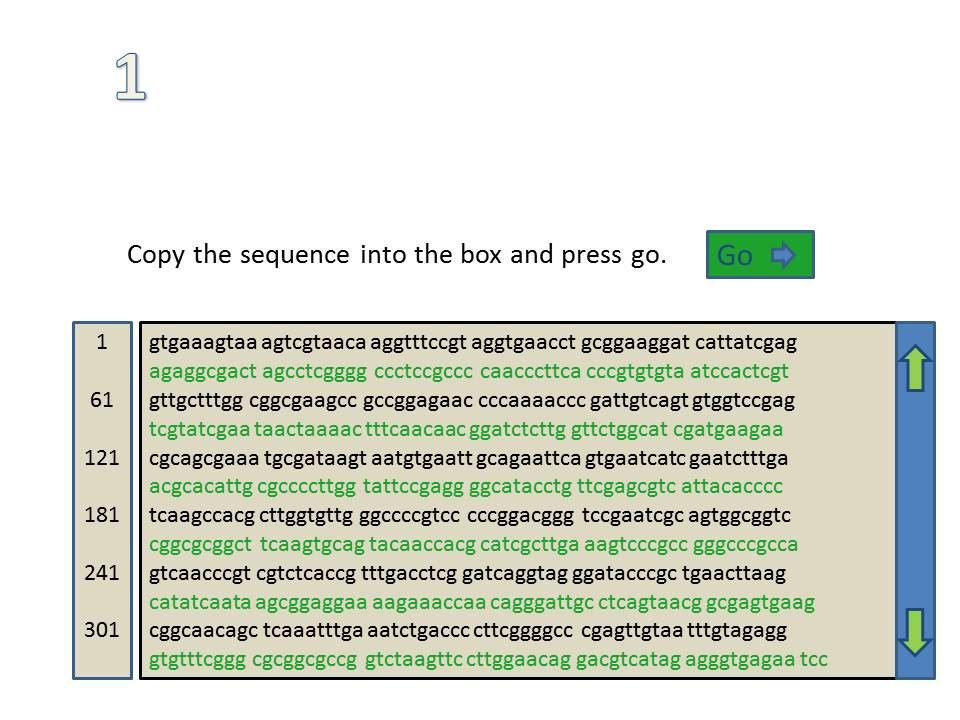
\includegraphics[width=0.6\textwidth]{./images/UiDes/Slide1.JPG}
    \caption{
      \label{fig:UiDes:slide1}
      Initial design, Sequence entry
    }
  \end{center}
\end{figure}

\subsubsection{Sequence entry (figure \ref{fig:UiDes:slide1})}
The first slide shows the sequence entry screen, where the user copies
the DNA sequence on which to perform PCR into the provided box.
The complementary strand is generated automatically and shown in different 
colour. The numbers on the left show the index number at the start of the
corresponding line, as a way for the user to quickly find the part of
the sequence to be amplified in the next stage and to provide better
orientation in the sequence altogether.
Scrolling through the sequence is performed either by pressing the arrow buttons
on the right or using scrolling with the mouse.
Once the user is content with the sequence entered, he can press the
"Go" button to advance to the next stage.

\begin{figure}[h]
  \begin{center}
	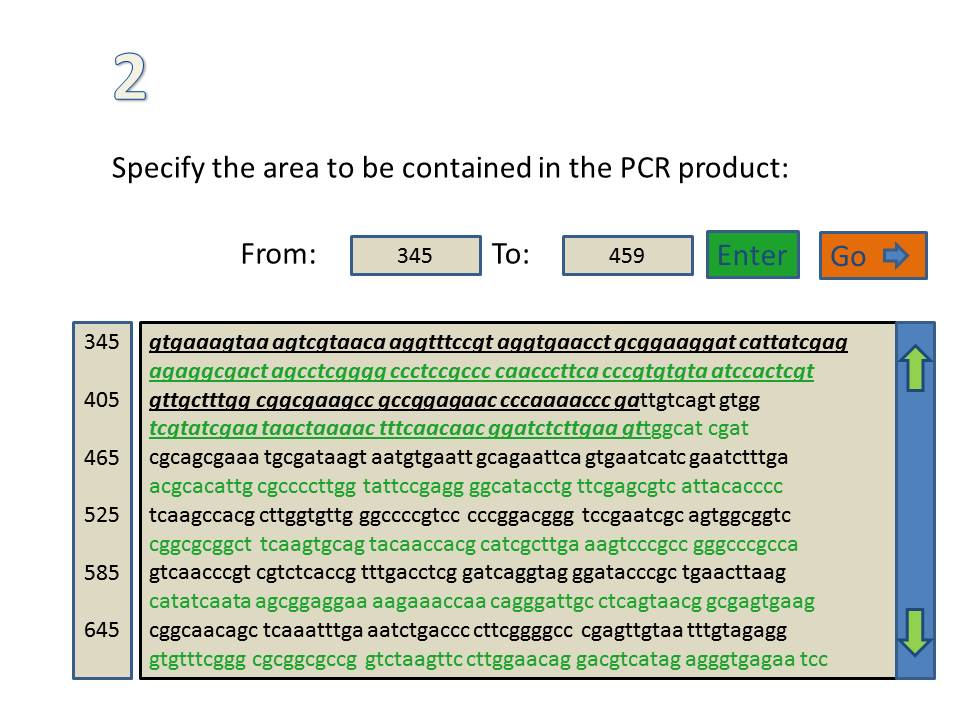
\includegraphics[width=0.6\textwidth]{./images/UiDes/Slide2.JPG}
    \caption{
      \label{fig:UiDes:slide2}
      Initial design,Specification of target area
    }
  \end{center}
\end{figure}


\subsubsection{Specification of target area (figure \ref{fig:UiDes:slide2})}
The second slide shows the selection of the DNA sequence part to be
amplified by PCR.
The user enters the first and the last base indices in the ``From" and
``To" text fields respectively, and the chosen area is highlighted
after the user presses the ``Enter" button.
All of the previously introduced functions of the UI, including DNA
sequence editing, are present at this stage also.
When the user is content with the area specified, they can press the
``Go" button to advance to the next stage.
The ``Go" button color is changed to clearly differentiate from the
``Enter" button.

\begin{figure}[h]
  \begin{center}
	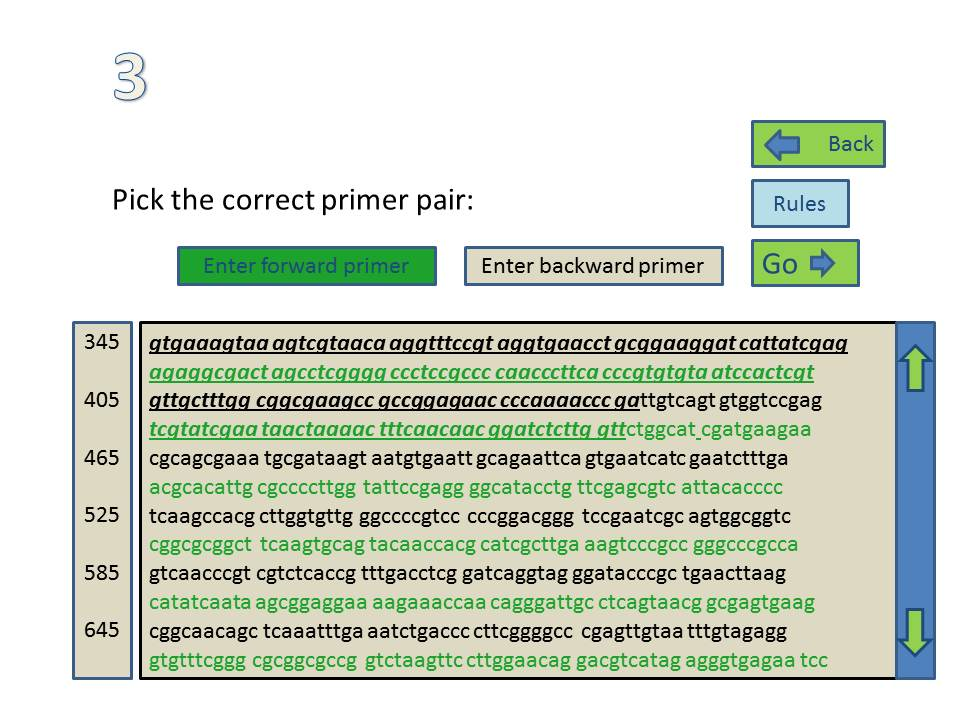
\includegraphics[width=0.6\textwidth]{./images/UiDes/slide3.jpg}
    \caption{
      \label{fig:UiDes:slide3}
      Initial design, Primer selection - initial screen
    }
  \end{center}
\end{figure}


\subsubsection{Primer selection (figure \ref{fig:UiDes:slide3})}

The user is prompted to copy/paste or type the forward and the reverse
primers into their respective text fields located above the sequence.
At the time of the interface being designed the team was still
becoming accustomed to the terminology involved so the design
mistakenly shows ``Backward'' primer instead of the correct
``Reverse''.
The rules of primer design can be viewed by pressing the ``Rules''
button.
If the user decides to change the target area or the sequence itself,
they can go back to the previous stage by pressing the ``Back'' button. 



When the user has entered the primers into their respective boxes, as
shown in figure \ref{fig:UiDes:slide3}, the user can press the ``Go'' button
to go to the next stage if the primers are correct, or be shown an
error message if they are not.

\begin{figure}[h]
  \begin{center}
	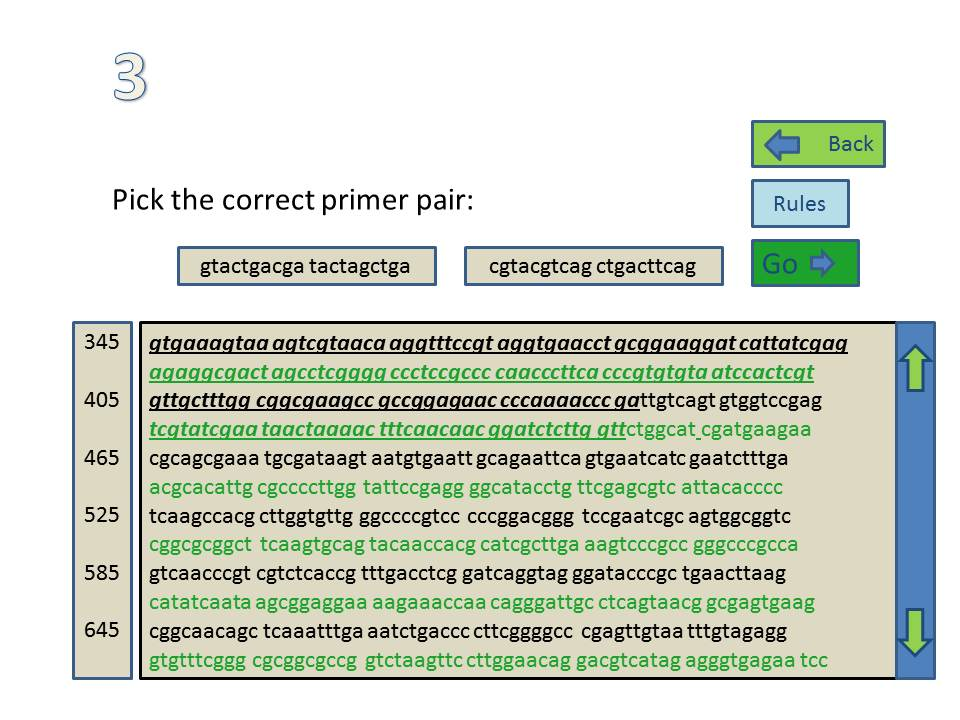
\includegraphics[width=0.6\textwidth]{./images/UiDes/Slide4.JPG}
    \caption{
      \label{fig:UiDes:slide4}
      Initial design, Primer selection - primers entered
    }
  \end{center}
\end{figure}

\begin{figure}[h]
  \begin{center}
	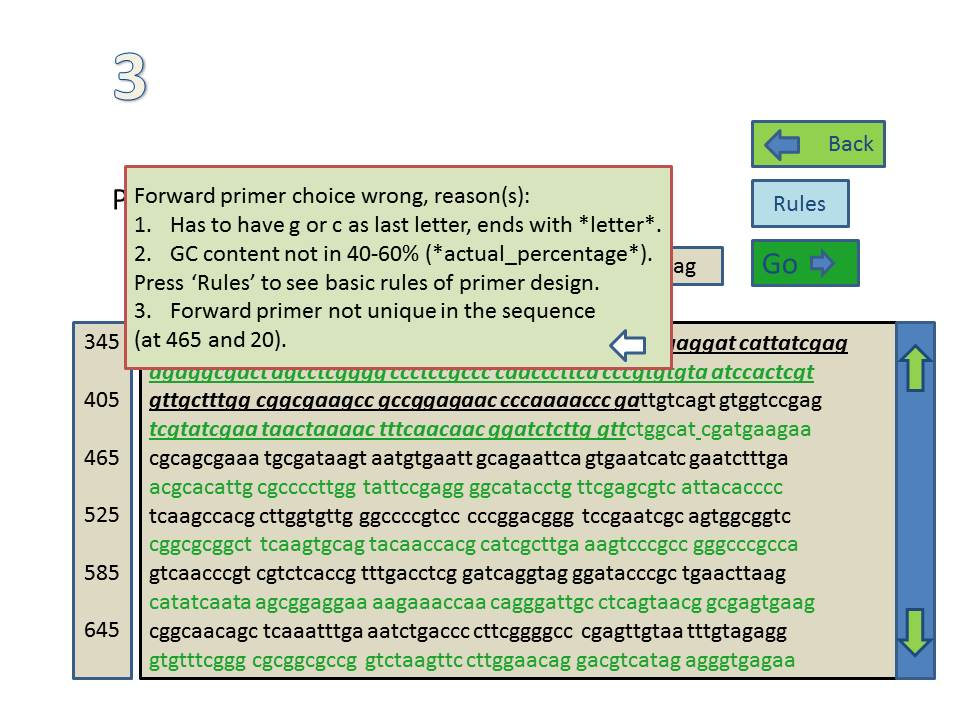
\includegraphics[width=0.6\textwidth]{./images/UiDes/slide5.jpg}
    \caption{
      \label{fig:UiDes:slide5}
      Initial design, Primer selection - error message
    }
  \end{center}
\end{figure}

Each primer is checked for correctness according to the primer design
rules and the user is shown a message explaining why their chosen primer
is incorrect for the target sequence.
In the case that both primers are incorrect, a separate list of errors
is shown for each one.
The user can then press the white arrow button to go back to selecting
the primers again.



\subsubsection{Melting temperature check (figure \ref{fig:UiDes:slide6})}
The last slide shows the primers chosen by the user still in their
respective boxes and their melting temperatures just below.
Both temperatures must be in the range of 50 to 60\degree C for
PCR to work, so if they are not the user is suggested going back to
the previous screen and selecting a different primer pair.
As before, pressing ``Back'' will take the user to a previous stage.
The user is also advised to visit the NCBI website \cite{ncbi} and
performing primer blast on his selected primers to check them for
specificity. Lastly, pressing the "Go" button will open a new window
with an animation of PCR in action.

\begin{figure}[h]
  \begin{center}
	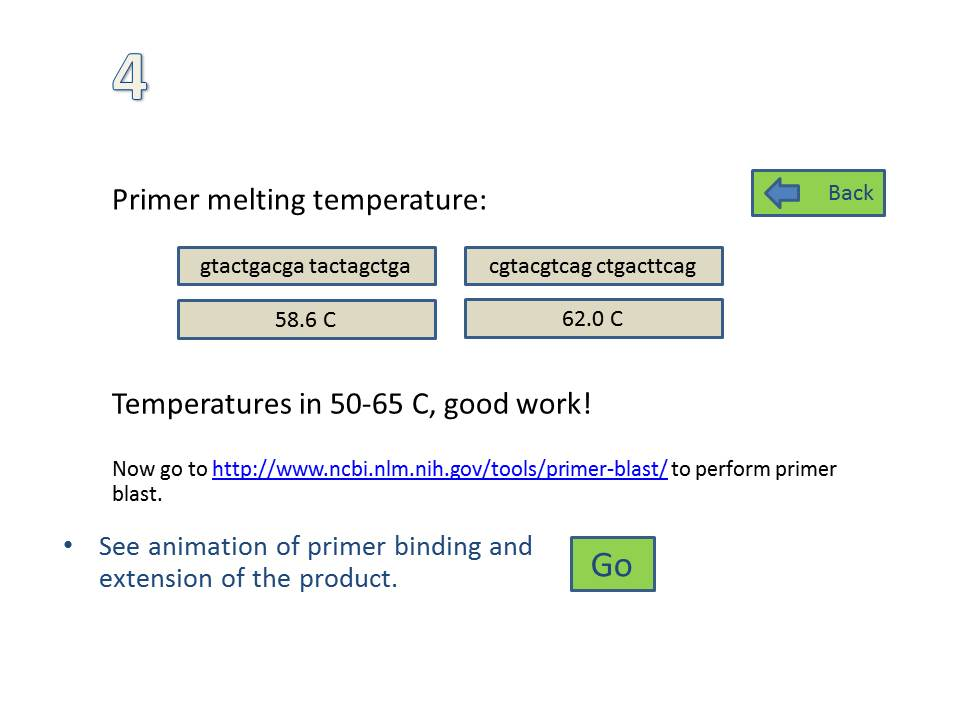
\includegraphics[width=0.6\textwidth]{./images/UiDes/Slide6.JPG}
    \caption{
      \label{fig:UiDes:slide6}
      Initial design, Primer melting temperatures
    }
  \end{center}
\end{figure}

